\definecolor{azul_custom}{RGB}{66,240,209}
\definecolor{lila_custom}{RGB}{201,69,254}
\definecolor{naranja_custom}{RGB}{255,148,0}


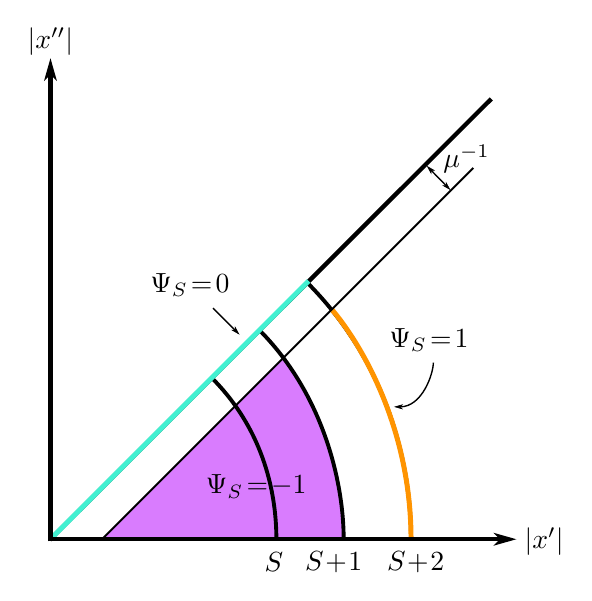
\begin{tikzpicture}[y=0.80pt, x=0.80pt, yscale=-1.000000, xscale=1.000000, inner sep=0pt, outer sep=0pt]


%region-down
\path[scale=0.938,fill=lila_custom, opacity = 0.7, line width=0.400pt] (248.0459,242.6193) ..
controls (275.7060,284.1286) and (276.2013,310.5581) .. (276.7985,330.5197) ..
controls (233.8448,330.5197) and (216.3370,330.5469) .. (160.2334,330.5469) ..
controls (186.2822,304.6380) and (219.4410,271.2569) .. (248.0459,242.6193) --
cycle;



%big circle
\path[draw=black,line join=miter,line cap=butt,line width=1.4pt]
(243.0000,193.8560) .. controls (275.7522,226.7370) and (289.9164,269.7115) ..
(289.9164,309.8622);

%big circle2
\path[draw=naranja_custom,line join=miter,line cap=butt,line width=1.8pt]
(243.0000+11,193.8560+12) .. controls (275.7522-9,226.7370-6) and (289.9164,258.7115) ..
(289.9164,309.8622);

%medium circle
\path[draw=black,line join=miter,line cap=butt,line width=1.4pt]
(221.4938,215.3997) .. controls (250.7785,244.9692) and (259.4986,284.9193) ..
(259.4986,309.8622);

%small circle    
\path[draw=black,line join=miter,line cap=butt,line width=1.4pt]
(199.9500,236.9435) .. controls (222.0483,259.0975) and (229.1002,286.5606) ..
(229.1002,309.8622);

%cone   
\path[draw=black,line join=miter,line cap=butt,miter limit=4.00,even odd
rule,line width=1.57pt] (126.7629,310.0643) -- (326.1869,110.8844);

%cone+1    
\path[draw=black,line join=miter,line cap=butt,even odd rule,line width=0.704pt]
(150.2563,309.8481) -- (318.0555,142.0518);


%Linea Cota
\path[draw=black,line join=miter,line cap=butt,line width=0.5pt]
(298.3343,142.4919) -- (306.3936,150.7321);


%Flecha Izquierda Cota
\path[draw=black,fill=black,even odd rule,line width=0.200pt]
(298.9657,143.1375) -- (300.2914,143.1522) -- (297.3269,141.4619) --
(298.9510,144.4632) -- cycle;

%Flecha Derecha Cota
\path[draw=black,fill=black,even odd rule,line width=0.200pt]
(305.7622,150.0865) -- (304.4364,150.0718) -- (307.4010,151.7621) --
(305.7769,148.7608) -- cycle;

%Cota naranja
\path[draw=black,line join=miter,line cap=butt,line width=0.5pt]
(300, 230) .. controls (300, 235) and (295, 250) ..
(285, 250);

%Flecha cota naranja
\path[draw=black,fill=black,even odd rule,line width=0.200pt]
(285, 250) -- (285+0.9375, 250+0.9375) -- (285-2.3437, 250) --
(285+0.9375, 250-0.9375) -- cycle;

%Flecha Cono Cota (221.4938,215.3997)
\path[draw=black,fill=black,even odd rule,line width=0.200pt]
(210.4938,215.3997) -- (210.4938-1.3258,215.3997-0.0147) -- (210.4938+1.6388,215.3997+1.6759) --
(210.4938+0.0147,215.3997-1.3257) -- cycle;

%Linea Cota
\path[draw=black,line join=miter,line cap=butt,line width=0.5pt]
(210.4938,215.3997) -- (210.4938-10,215.3997-10);

%Linea Cono
\path[draw=azul_custom,line join=miter,line cap=butt,line width=1.8pt]
(126.7629+1,310.0643-1) -- (243.0000+0.7,193.8560-0.7);

%x-axis    
\path[draw=black,line join=miter,line cap=butt,line width=1.5pt]
(126.5055,309.8063) -- (330.4872,309.8063);

%x-axis cap    
\path[draw=black,fill=black,even odd rule,line width=0.497pt]
(330.4872,309.8063) -- (328.1493,312.1289) -- (336.3320,309.8063) --
(328.1493,307.4838) -- cycle;

%y-axis
\path[draw=black,line join=miter,line cap=butt,line width=1.5pt]
(127.0562,310.75) -- (127.0562,99.5223);

%y-axis cap    
\path[draw=black,fill=black,even odd rule,line width=0.497pt] (127.0562,99.5223)
-- (129.3788,101.8602) -- (127.0562,93.6775) -- (124.7336,101.8602) -- cycle;


\node at (315,138) {\normalsize $\mu^{-1}$};
\node at (127,85) {\normalsize $|x''|$};
\node at (350, 311) {\normalsize $|x'|$};
\node at (228,320) {\normalsize $S$};
\node at (255, 320) {\normalsize $S\!+\!1$};
\node at (292, 320) {\normalsize $S\!+\!2$};
\node at (334, 101) {\normalsize $\ccal$};
\node at (298, 220) {\normalsize $\Psi_S\! = \!1$};
\node at (220, 286) {\normalsize $\Psi_S\! = \!-1$};
\node at (190, 195) {\normalsize $\Psi_S\! = \!0$};


\end{tikzpicture}